\documentclass{article}
\usepackage{graphicx}
\usepackage{listings}
\usepackage{color}
\usepackage{float}
\usepackage{amsmath}
\usepackage{geometry}
\usepackage{hyperref}
\usepackage{amssymb}

\geometry{a4paper, margin=1in}

% Code highlighting colors
\definecolor{codegreen}{rgb}{0,0.6,0}
\definecolor{codegray}{rgb}{0.5,0.5,0.5}
\definecolor{codepurple}{rgb}{0.58,0,0.82}
\definecolor{backcolour}{rgb}{0.95,0.95,0.92}

\lstdefinestyle{mystyle}{
    backgroundcolor=\color{backcolour},   
    commentstyle=\color{codegreen},
    keywordstyle=\color{codepurple},
    numberstyle=\tiny\color{codegray},
    stringstyle=\color{codegreen},
    basicstyle=\ttfamily\footnotesize,
    breakatwhitespace=false,         
    breaklines=true,                 
    captionpos=b,                    
    keepspaces=true,                 
    numbers=left,                    
    numbersep=5pt,                  
    showspaces=false,                
    showstringspaces=false,
    showtabs=false,                  
    tabsize=2
}

\lstset{style=mystyle}

\title{Digital Clock Implementation with Arduino}
\author{EE24BTECH11024 - Abhimanyu Koushik}
\date{\today}

\begin{document}

\maketitle

\tableofcontents
\newpage

\section{Introduction}
This report describes the design, implementation, and analysis of a digital clock using an \textit{Arduino Uno} microcontroller, \textit{7-segment displays}, and \textit{multiplexing techniques}. The project employs AVR-GCC programming for efficient control and accurate timekeeping.

\section{Objectives}
The primary objectives of this project are:
\begin{itemize}
    \item To create a digital clock capable of displaying hours, minutes, and seconds.
    \item To use \textit{multiplexing} techniques for reducing the number of required microcontroller pins.
    \item To implement precise time management using \textit{Timer1 interrupts}.
    \item To demonstrate AVR-GCC direct register manipulation for efficient hardware control.
\end{itemize}

\section{Materials Required}
\begin{itemize}
    \item \textit{Arduino Uno} board (ATmega328P)
    \item Six \textit{7-segment displays}
    \item \textit{7447 BCD-to-7-segment decoders}
    \item \textit{180}$\Omega$ \textit{resistors} (current limiting resistors)
    \item \textit{Push buttons} (for time adjustments)
    \item Breadboard and jumper wires
    \item Power supply or USB connection for the Arduino
\end{itemize}

\section{Circuit Description}
The clock uses six 7-segment displays to represent \textit{HH:MM:SS}. The digits are arranged as follows:
\[
\text{{HH:MM:SS}} = \text{{Hour Tens}} + \text{{Hour Units}} + \text{{Minute Tens}} + \text{{Minute Units}} + \text{{Second Tens}} + \text{{Second Units}}
\]

\subsection{Wiring Configuration}
\begin{figure}[H]
    \centering
    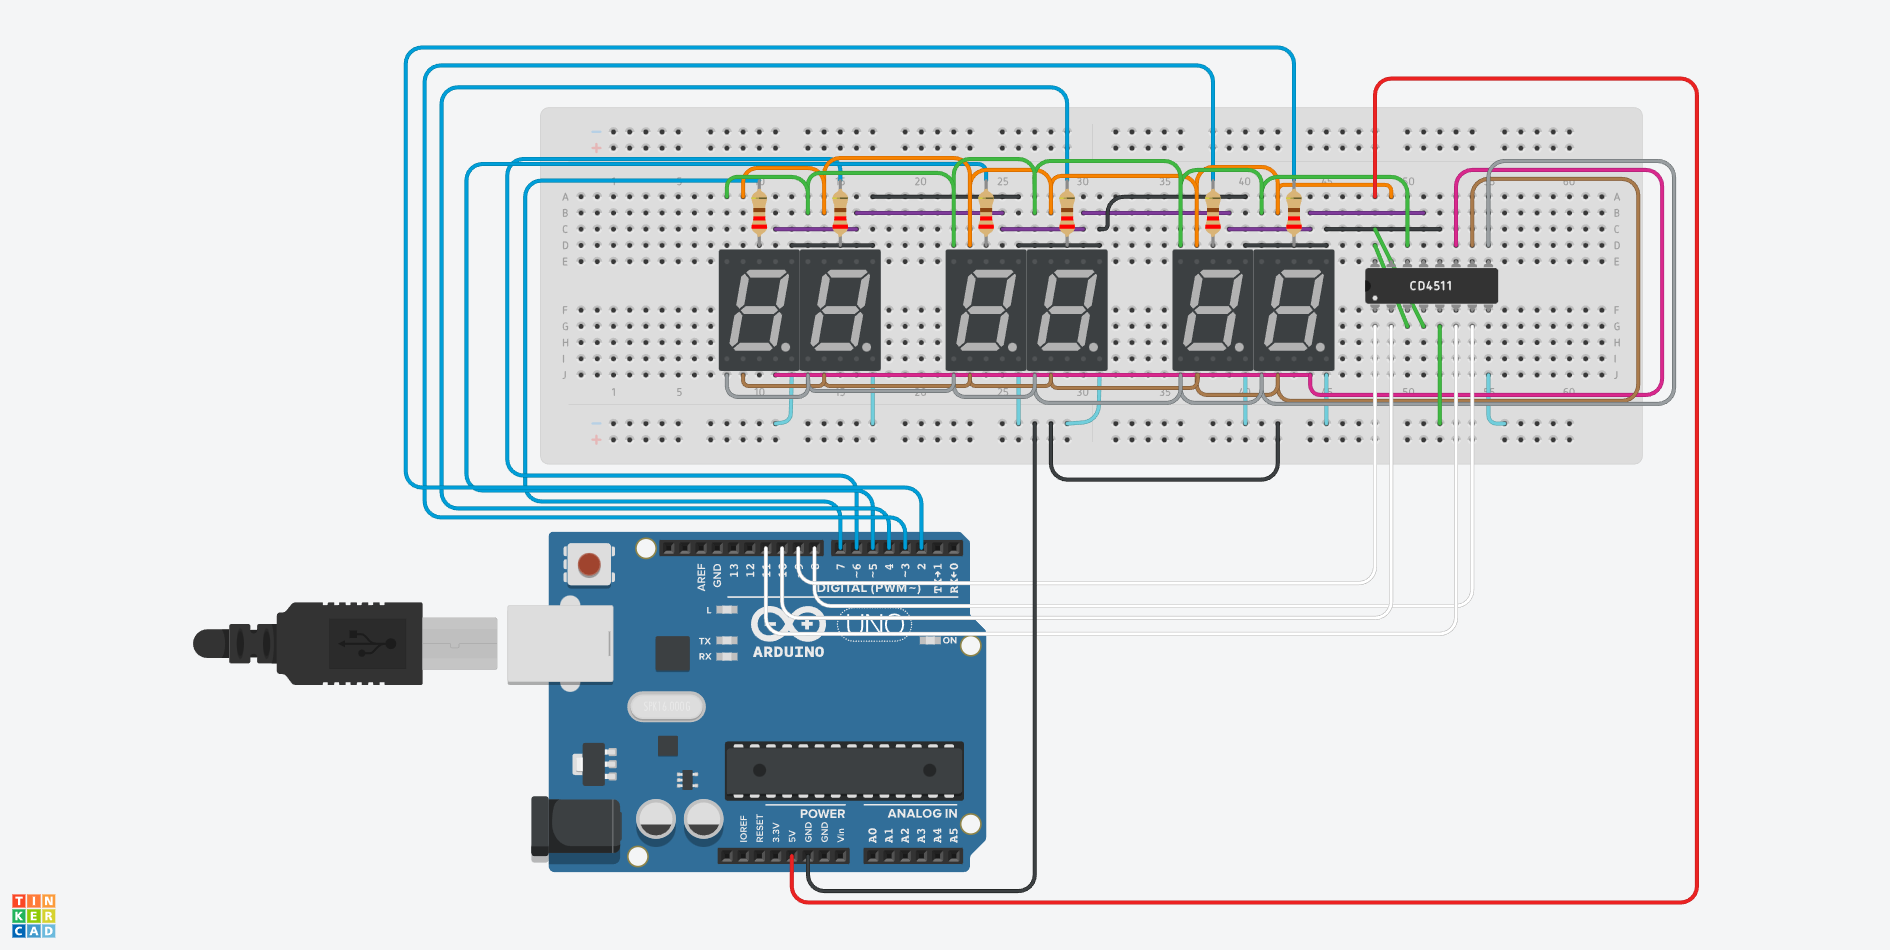
\includegraphics[width=\textwidth]{figs/Clock.jpg}
    \caption{Digital Clock Circuit using Arduino and 7-segment displays}
\end{figure}

\subsection{Pin Diagrams}

\begin{figure}[H]
    \centering
    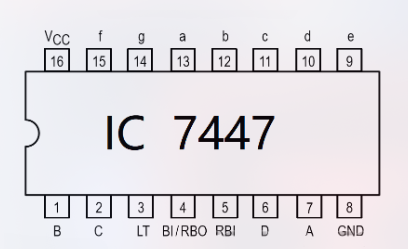
\includegraphics[width=0.6\textwidth]{figs/7447_pinout.jpg}
    \caption{7447 BCD-to-7-segment Decoder Pinout}
\end{figure}

\begin{figure}[H]
    \centering
    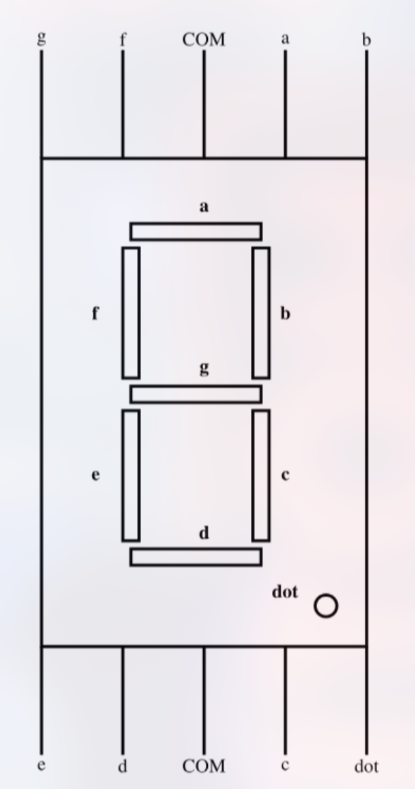
\includegraphics[width=0.3\textwidth]{figs/7seg_pinout.jpg}
    \caption{7-segment Display Pinout}
\end{figure}

\subsection{Connections}

\subsubsection{7447 Decoder to Arduino Connections}
\begin{itemize}
    \item D2 → A (LSB) on 7447
    \item D3 → B on 7447
    \item D4 → C on 7447
    \item D5 → D (MSB) on 7447
    \item GND → GND (Common ground)
\end{itemize}

\subsubsection{7447 to 7-segment Display Connections}
\begin{itemize}
    \item 7447 Pin 9 → Segment E
    \item 7447 Pin 10 → Segment D
    \item 7447 Pin 11 → Segment C
    \item 7447 Pin 12 → Segment B
    \item 7447 Pin 13 → Segment A
    \item 7447 Pin 14 → Segment G
    \item 7447 Pin 15 → Segment F
\end{itemize}

\subsubsection{7-segment Display to Arduino Connections}
\begin{itemize}
    \item A0 → Display 1 Common Anode
    \item A1 → Display 2 Common Anode
    \item A2 → Display 3 Common Anode
    \item A3 → Display 4 Common Anode
    \item A4 → Display 5 Common Anode
    \item A5 → Display 6 Common Anode
\end{itemize}

\section{Working Principle}
The clock uses \textit{multiplexing} to drive multiple 7-segment displays while reducing the required number of pins. The Arduino cycles through each display quickly (approximately every 2ms), creating the illusion of simultaneous illumination.

\subsection{Timing and Multiplexing}
The \textit{Timer1 interrupt} triggers every second to update the clock values. The display refresh rate is approximately:
\[
\text{{Refresh rate}} = \frac{1}{12\text{ms}} \approx 83\text{Hz}
\]

\section{Challenges and Solutions}
\begin{itemize}
    \item Flickering: Increasing the refresh rate resolved flickering issues.
    \item Time accuracy: Timer1 was configured with a prescaler of 1024 to ensure accurate 1-second timekeeping.
    \item Pin limitations: Multiplexing allowed the use of fewer pins by controlling each digit sequentially.
\end{itemize}

\section{Conclusion}
This project successfully demonstrates the implementation of a digital clock using \textit{AVR-GCC} programming on an \textit{Arduino Uno}. The use of multiplexing reduces the required number of pins, while Timer1 interrupts ensure accurate timekeeping. The clock displays \textit{hours, minutes, and seconds} using six 7-segment displays and a 7447 BCD-to-7-segment decoder.

\section{Source Code and Documentation}
The complete source code and documentation are available on GitHub:
\begin{center}
\href{https://github.com/AbhimanyuKoushik/nice_stuff/tree/main/codes/Arduino/Clock/clock_Decoder}{https://github.com/AbhimanyuKoushik/Digital-Clock-Arduino}
\end{center}

\end{document}
